% act_1.6
\subsection{Joint PD control $+$ gravity compensation}
The objective of this activity is display the UR5 robot on rviz and control the motion of its joints with a PD with gravity compensation control method. The simulation starts with the initial joint configuration $\begin{bmatrix} \pi & -\frac{\pi}{8} & -\frac{\pi}{6} & 0.0 & 0.0 & 0.0 \end{bmatrix}$ rad and then move the second and fifth joints of the UR5 robot. On one hand, the two joints will maintain the initial configuration during first $2$ seconds and follow a step reference during last $3$ seconds. On the other hand, the two joints will move following a sinusoidal trajectory during first $4$ seconds and maintain a constant joint position during last second. The performance of the control method will be evaluated in next subsections.


\subsubsection{Step reference}
The Algorithm \ref{lst:joint_PD_gravity_compensation_control_method_step} control the movements of second and fifth joints of the UR5 robot to follow a step reference trajectory. In this file, the PD with gravity compensation control method is configured with $K_p=300$ $\mathrm{\frac{N.m}{rad}}$ and $K_d= 20 $ $\mathrm{\frac{N.m.s}{rad}}$. Figure \ref{fig:act_1.6_step_joint_position} shows the tracking performance of each joint of the UR5 robot. On one hand, the second joint ($\mathrm{q}_2$) presents overshoot ($15\%$) and steady state error close to $0$ rad. On the other hand, the fifth joint ($\mathrm{q}_5$)presents overshoot close to $0\%$ and steady state error close to $0$ rad. The variation of the temporal parameters of each joint is due to the control gains and the physical characteristics of the system. On one hand, the second joint must lift more mass than the fifth joint; and in the same way, the end effector of the robot is further from the second joint than from the fifth joint. In this context, the torque generated by robot's weight is greater in the second joint. On the other hand, the tracking error at transient state is due to the effect of Coriolis and centripetal forces. On the other hand, the tracking error at steady state is close to $0$ rad due to gravity term in control law is compensating the forces generated by UR5 robot weight. Finally, the Figure \ref{fig:act_1.6_step_g} show the variation of the gravity term ($g$) of the control method with a step reference. 

\begin{lstlisting}[language=Python,caption={Move the second and fifth joint of UR5 robot with the requirement motion of activity 1.6.1}, label={lst:joint_PD_gravity_compensation_control_method_step}]
# =========================
#   Configuration of node
# =========================
# create a node: 
rospy.init_node("node_joint_PD_control_gravity_compensation")

# public in topic /joint_states	to send joint data	
pub = rospy.Publisher('joint_states', JointState, queue_size=1000)

# loop rate (in Hz)
rate 	= rospy.Rate(1000)		# 100 [Hz]
dt 		= 1e-3					# 10  [ms]

# object(message) type JointState
jstate = JointState()

# ==========================================
#   Set initial joint configuration of UR5
# ==========================================
# initial configuration: position, velocity and acceleration 
q0 =   np.array([np.pi, -np.pi/8,  -np.pi/6, 0.0, 0.0, 0.0])
dq0 =  np.array([0.0, 0.0, 0.0, 0.0, 0.0, 0.0]) 
ddq0 = np.array([0.0, 0.0, 0.0, 0.0, 0.0, 0.0]) 

# desired trajectory: position, velocity and acceleration
q_des =   np.array([np.pi, -np.pi/8,  -np.pi/6, 0.0, 0.0, 0.0]) 
dq_des =  np.array([0.0, 0.0, 0.0, 0.0, 0.0, 0.0]) 
ddq_des = np.array([0.0, 0.0, 0.0, 0.0, 0.0, 0.0]) 

# measured trajectory: position, velocity and acceleration
q =   np.array([np.pi, -np.pi/8,  -np.pi/6, 0.0, 0.0, 0.0])
dq =  np.array([0.0, 0.0, 0.0, 0.0, 0.0, 0.0]) 
ddq = np.array([0.0, 0.0, 0.0, 0.0, 0.0, 0.0]) 

# ===========================
#   UR5 robot configuration
# ===========================
# joints name of UR5 robot
jnames = ['shoulder_pan_joint', 'shoulder_lift_joint', 'elbow_joint','wrist_1_joint', 'wrist_2_joint', 'wrist_3_joint']

# number of degress of freedom
ndof = 6
# the class robot load the ur5.urdf
ur5_robot = Robot(ndof,q0, dq0, dt)
# create inertia matrix 
M = np.zeros([ndof,ndof])
# create nonlinear effects vector
b = np.zeros(ndof)
# create gravity vector
g = np.zeros(ndof)

# ===============================
#   PD controller configuration
# ===============================
# proportional gain
kp = 300*np.ones(ndof)
# derivative gain
kd = 20*np.ones(ndof)
# control vector
tau = np.zeros(ndof)    

#===============
#   Simulation
#===============
t = 0.0             # [sec] 
sim_duration = 5.0  # [sec]
step_start = 2.0    # [sec]

while not rospy.is_shutdown():
    # generate step reference after 2 seconds
    if t>=step_start:
        # second link
        q_des[1], dq_des[1], ddq_des[1] = step_reference_generator(q0[1], -0.4)
        # fifth link
        q_des[4], dq_des[4], ddq_des[4] = step_reference_generator(q0[4], 0.5)

    # error: position and velocity
    e 	=  q_des - q
    de 	=  dq_des - dq    
    
    # compute gravitational effects vector
    g = ur5_robot.get_g()

    # PD control method + gravity compensation
    tau = np.multiply(kp, e) + np.multiply(kd, de) + g
    
    # send control signal
    ur5_robot.send_control_command(tau)
    # update states
    q, dq, ddq = ur5_robot.read_joint_position_velocity_acceleration()

    # publish message
    jstate.header.stamp = rospy.Time.now()
    jstate.name 		= jnames			# Joints position name
    jstate.position 	= q
    jstate.velocity 	= dq
    pub.publish(jstate)

    # update time
    t = t + dt
	# stop simulation
    if t>=sim_duration:
        print("stopping rviz ...")
        break
    rate.sleep()

\end{lstlisting}

\begin{figure}[H]
	\centering
	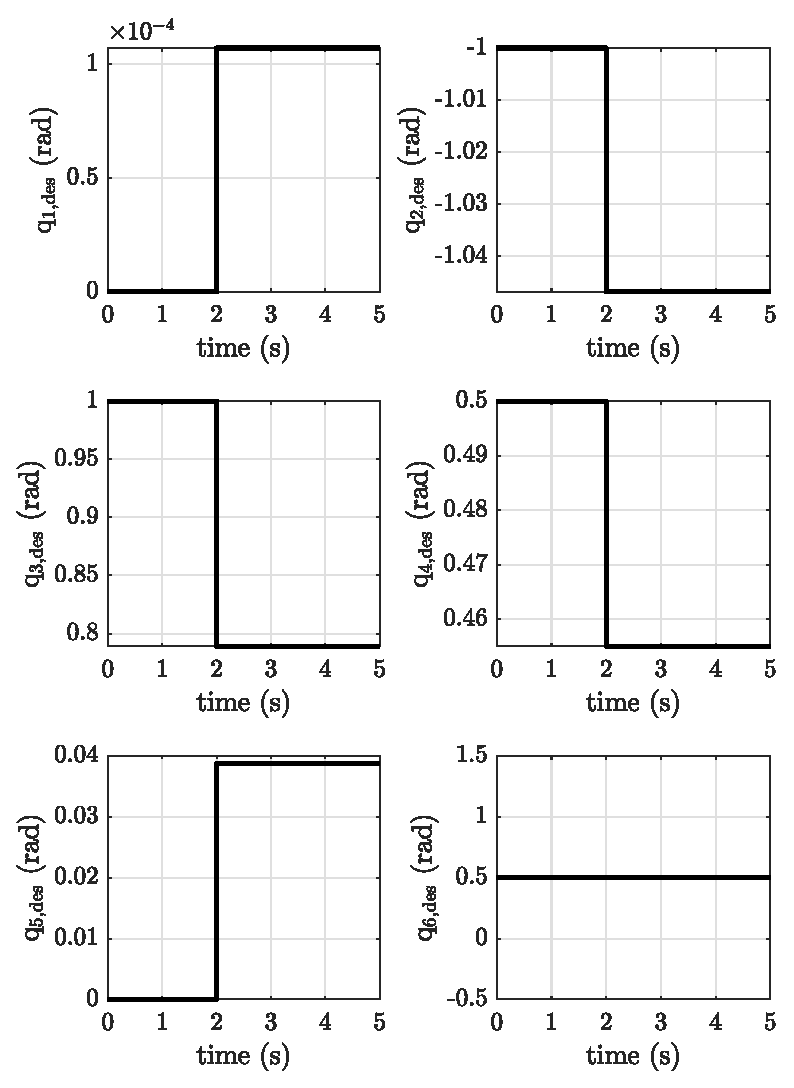
\includegraphics{images/act_1.6_step/joint_position.eps}
	\caption{Angular position of each joint of UR5 robot with Algorithm \ref{lst:joint_PD_gravity_compensation_control_method_step}.}
	\label{fig:act_1.6_step_joint_position}
\end{figure}
\begin{comment}
\begin{figure}[H]
	\centering
	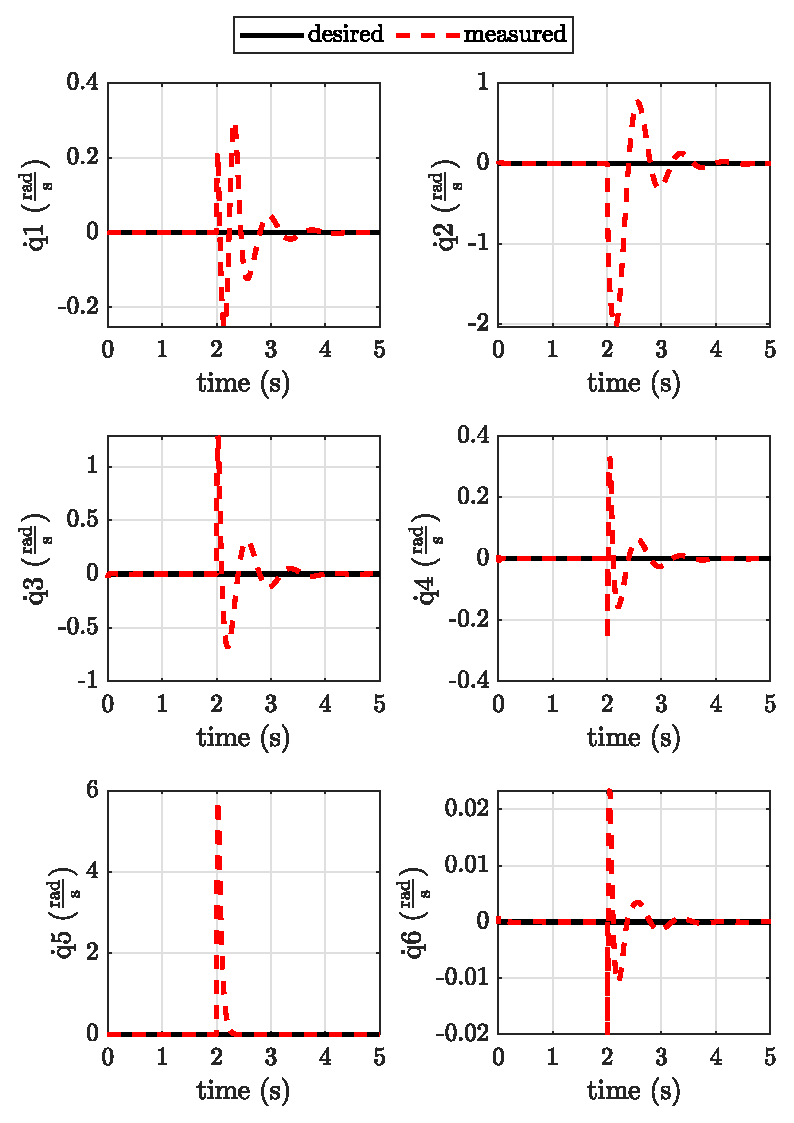
\includegraphics{images/act_1.6_step/joint_velocity.eps}
	\caption{Angular velocity of each joint of UR5 robot with Algorithm \ref{lst:joint_PD_gravity_compensation_control_method_step}.}
	\label{fig:act_1.6_step_joint_velocity}
\end{figure}

\begin{figure}[H]
	\centering
	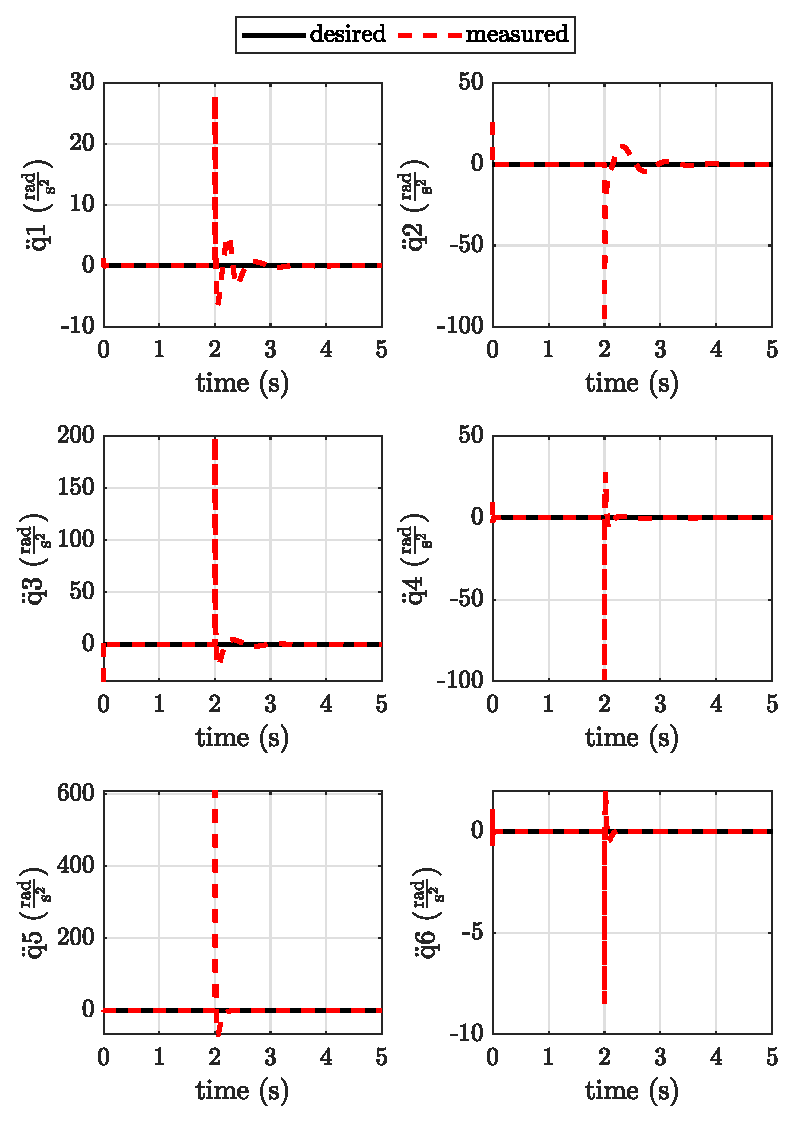
\includegraphics{images/act_1.6_step/joint_acceleration.eps}
	\caption{Angular acceleration of each joint of UR5 robot with Algorithm \ref{lst:joint_PD_gravity_compensation_control_method_step}.}
	\label{fig:act_1.6_step_joint_acceleration}
\end{figure}
\end{comment}
\begin{figure}[H]
	\centering
	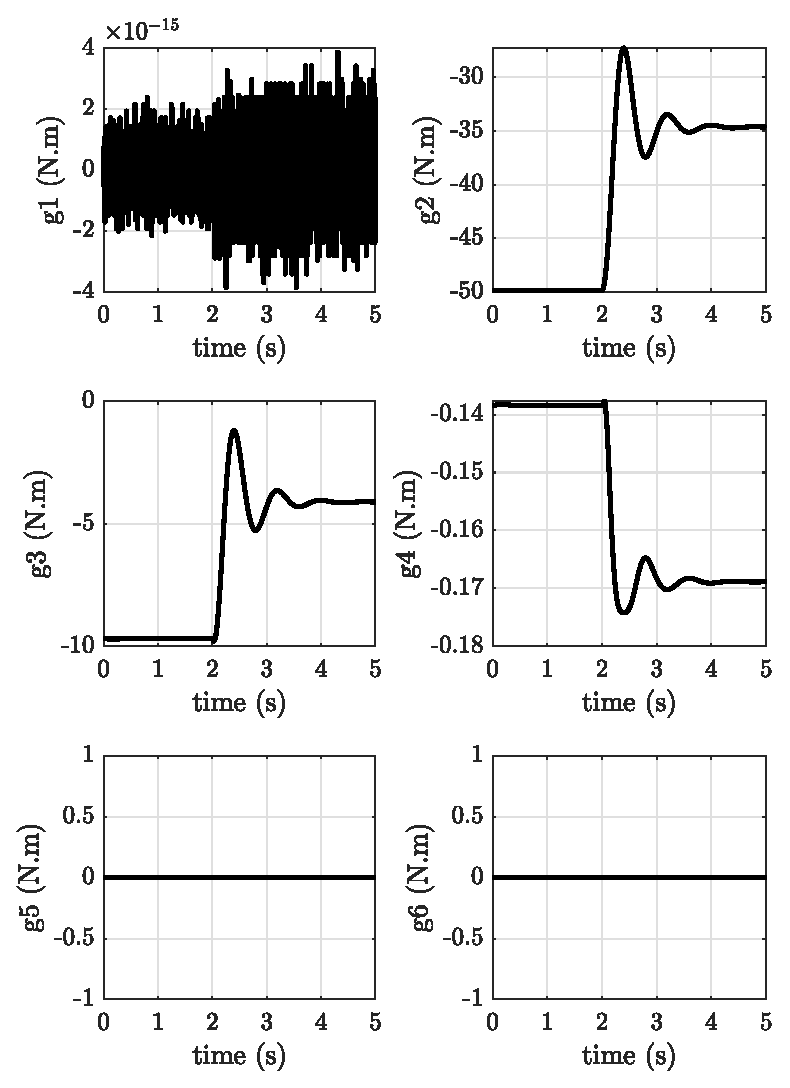
\includegraphics{images/act_1.6_step/g.eps}
	\caption{The gravity term ($g$) of the PD with gravity compensation control method when the reference of each joint is a constant value.}
	\label{fig:act_1.6_step_g}
\end{figure}



\newpage
\subsubsection{Sinusoidal reference}
The Algorithm \ref{lst:joint_PD_gravity_compensation_control_method_sinusoidal} control the movements of second and fifth joints of the UR5 robot to follow a sinusoidal reference trajectory. In this file, the PD with gravity compensation control method is configured with $K_p=300$ $\mathrm{\frac{N.m}{rad}}$ and $K_d= 20 $ $\mathrm{\frac{N.m.s}{rad}}$. Figure \ref{fig:act_1.6_sin_joint_position} shows the tracking performance of each joint of the UR5 robot. On one hand, the second joint ($\mathrm{q}_2$) presents overshoot ($15\%$) and steady state error close to $0$ rad. On the other hand, the fifth joint ($\mathrm{q}_5$)presents overshoot close to $0\%$ and steady state error close to $0$ rad. The variation of the temporal parameters of each joint is due to the control gains and the physical characteristics of the system. On one hand, the second joint must lift more mass than the fifth joint; and in the same way, the end effector of the robot is further from the second joint than from the fifth joint. In this context, the torque generated by robot's weight is greater in the second joint. On the other hand, the tracking error at transient state is due to the effect of Coriolis and centripetal forces. On the other hand, the tracking error at steady state is close to $0$ rad due to gravity term in control law is compensating the forces generated by UR5 robot weight. Finally, the Figure \ref{fig:act_1.6_sin_g} show the variation of the gravity term ($g$) of the control method when the reference of second and fifth joint is a sinusoidal trajectory. \vspace{5px}

\begin{lstlisting}[language=Python,caption={Move the second and fifth joint of UR5 robot with the requirement motion of activity 1.6.2}, label={lst:joint_PD_gravity_compensation_control_method_sinusoidal}]
# =========================
#   Configuration of node
# =========================
# create a node: 
rospy.init_node("node_joint_PD_control_gravity_compensation")

# public in topic /joint_states	to send joint data	
pub = rospy.Publisher('joint_states', JointState, queue_size=1000)

# loop rate (in Hz)
rate 	= rospy.Rate(1000)		# 100 [Hz]
dt 		= 1e-3					# 10  [ms]

# object(message) type JointState
jstate = JointState()

# ==========================================
#   Set initial joint configuration of UR5
# ==========================================
# initial configuration: position, velocity and acceleration 
q0 =   np.array([np.pi, -np.pi/8,  -np.pi/6, 0.0, 0.0, 0.0])
dq0 =  np.array([0.0, 0.0, 0.0, 0.0, 0.0, 0.0]) 
ddq0 = np.array([0.0, 0.0, 0.0, 0.0, 0.0, 0.0]) 

# desired trajectory: position, velocity and acceleration
q_des =   np.array([np.pi, -np.pi/8,  -np.pi/6, 0.0, 0.0, 0.0]) 
dq_des =  np.array([0.0, 0.0, 0.0, 0.0, 0.0, 0.0]) 
ddq_des = np.array([0.0, 0.0, 0.0, 0.0, 0.0, 0.0]) 

# measured trajectory: position, velocity and acceleration
q =   np.array([np.pi, -np.pi/8,  -np.pi/6, 0.0, 0.0, 0.0])
dq =  np.array([0.0, 0.0, 0.0, 0.0, 0.0, 0.0]) 
ddq = np.array([0.0, 0.0, 0.0, 0.0, 0.0, 0.0]) 

# ===========================
#   UR5 robot configuration
# ===========================
# joints name of UR5 robot
jnames = ['shoulder_pan_joint', 'shoulder_lift_joint', 'elbow_joint','wrist_1_joint', 'wrist_2_joint', 'wrist_3_joint']

# number of degress of freedom
ndof = 6
# the class robot load the ur5.urdf
ur5_robot = Robot(ndof,q0, dq0, dt)
# create inertia matrix 
M = np.zeros([ndof,ndof])
# create nonlinear effects vector
b = np.zeros(ndof)
# create gravity vector
g = np.zeros(ndof)

# ===============================
#   PD controller configuration
# ===============================
# proportional gain
kp = 300*np.ones(ndof)
# derivative gain
kd = 20*np.ones(ndof)
# control vector
tau = np.zeros(ndof)    

#===============
#   Simulation
#===============
t = 0.0             # [sec] 
sim_duration = 5.0  # [sec]
sine_duration = 4.0    # [sec]

while not rospy.is_shutdown():
    # generate sinusoidal joint reference
    if t<=sine_duration:
        # second link
        q_des[1], dq_des[1], ddq_des[1] = sinusoidal_reference_generator(q0[1], dq0[1], ddq0[1], 0.2, 1, t)
        last_q_des_1 = q_des[1]
        # fifth link
        q_des[4], dq_des[4], ddq_des[4] = sinusoidal_reference_generator(q0[4], dq0[4], ddq0[4], 0.4, 1.5, t)  
        last_q_des_4 = q_des[4]  
    else:   
        # second link
        q_des[1], dq_des[1], ddq_des[1] = step_reference_generator(0, last_q_des_1)
        # fifth link
        q_des[4], dq_des[4], ddq_des[4] = step_reference_generator(0 , last_q_des_4)
    # error: position and velocity
    e 	=  q_des - q
    de 	=  dq_des - dq    

    # compute gravitational effects vector
    g = ur5_robot.get_g()

    # PD control method + gravity compensation
    tau = np.multiply(kp, e) + np.multiply(kd, de) + g
    
    # send control signal
    ur5_robot.send_control_command(tau)
    # update states
    q, dq, ddq = ur5_robot.read_joint_position_velocity_acceleration()

    # publish message
    jstate.header.stamp = rospy.Time.now()
    jstate.name 		= jnames			# Joints position name
    jstate.position 	= q
    jstate.velocity 	= dq
    pub.publish(jstate)

    # update time
    t = t + dt
   
    # stop simulation
    if t>=sim_duration:
        print("stopping rviz ...")
        break
    rate.sleep()
\end{lstlisting}


\begin{figure}[H]
	\centering
	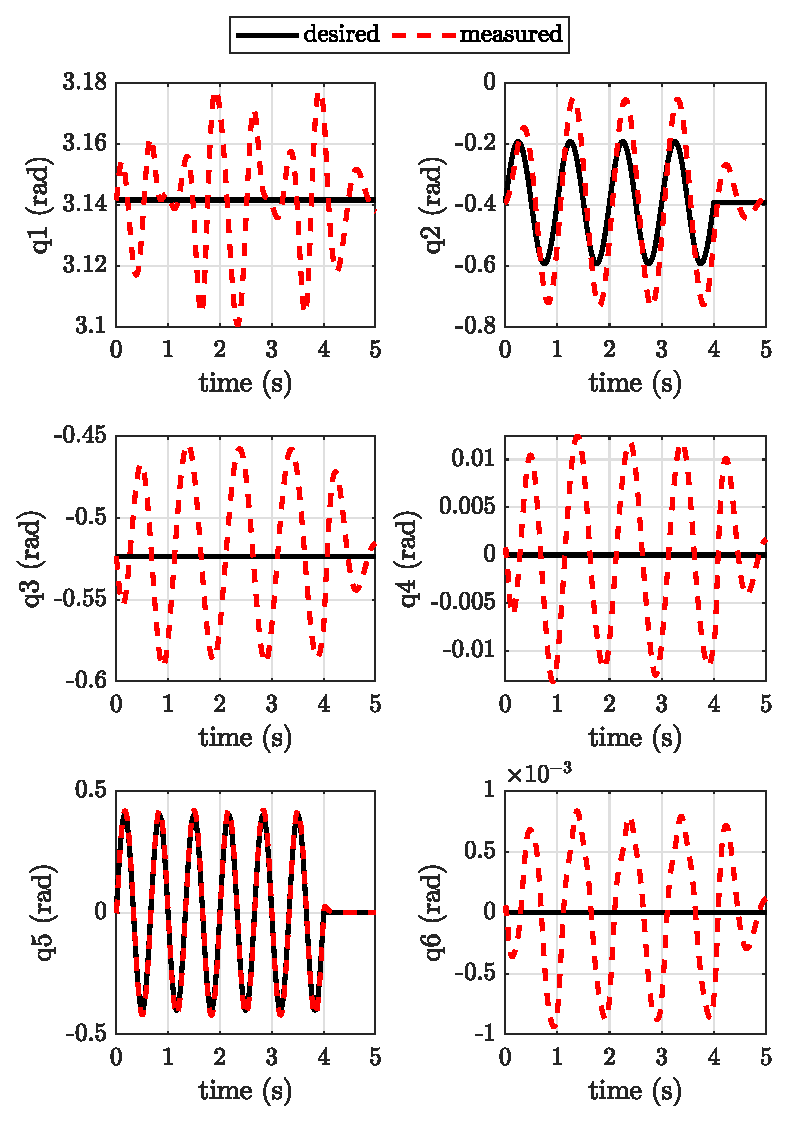
\includegraphics{images/act_1.6_sin/joint_position.eps}
	\caption{Angular position of each joint of UR5 robot with Algorithm \ref{lst:joint_PD_gravity_compensation_control_method_sinusoidal}.}
	\label{fig:act_1.6_sin_joint_position}
\end{figure}

\begin{comment}
\begin{figure}[H]
	\centering
	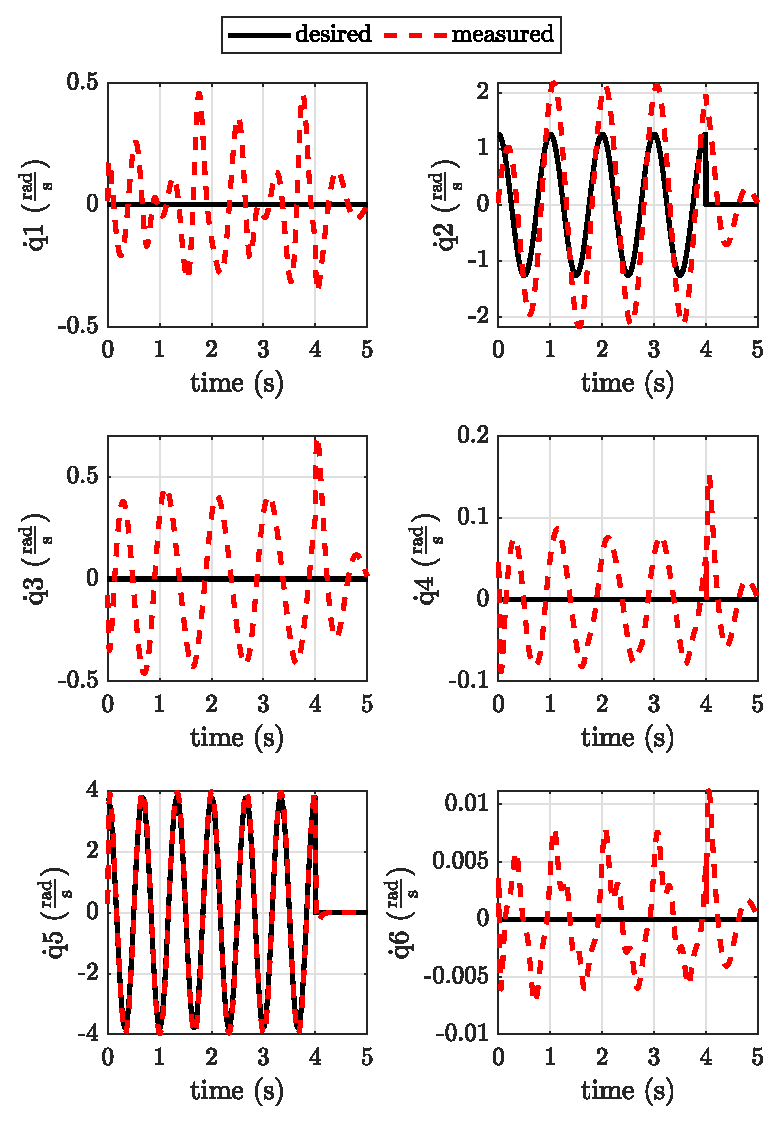
\includegraphics{images/act_1.6_sin/joint_velocity.eps}
	\caption{Angular velocity of each joint of UR5 robot with Algorithm \ref{lst:joint_PD_gravity_compensation_control_method_sinusoidal}.}
	\label{fig:act_1.6_sin_joint_velocity}
\end{figure}


\begin{figure}[H]
	\centering
	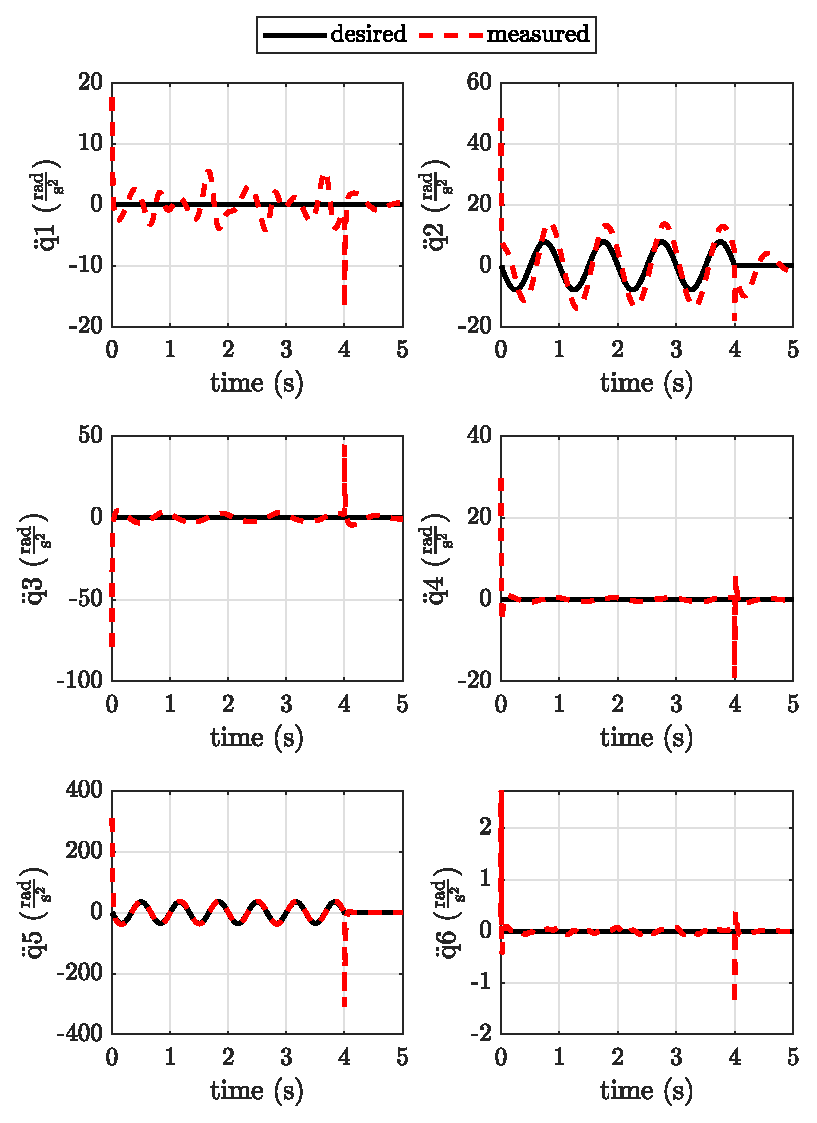
\includegraphics{images/act_1.6_sin/joint_acceleration.eps}
	\caption{Angular acceleration of each joint of UR5 robot with Algorithm \ref{lst:joint_PD_gravity_compensation_control_method_sinusoidal}.}
	\label{fig:act_1.6_sin_joint_acceleration}
\end{figure}
\end{comment}

\begin{figure}[H]
	\centering
	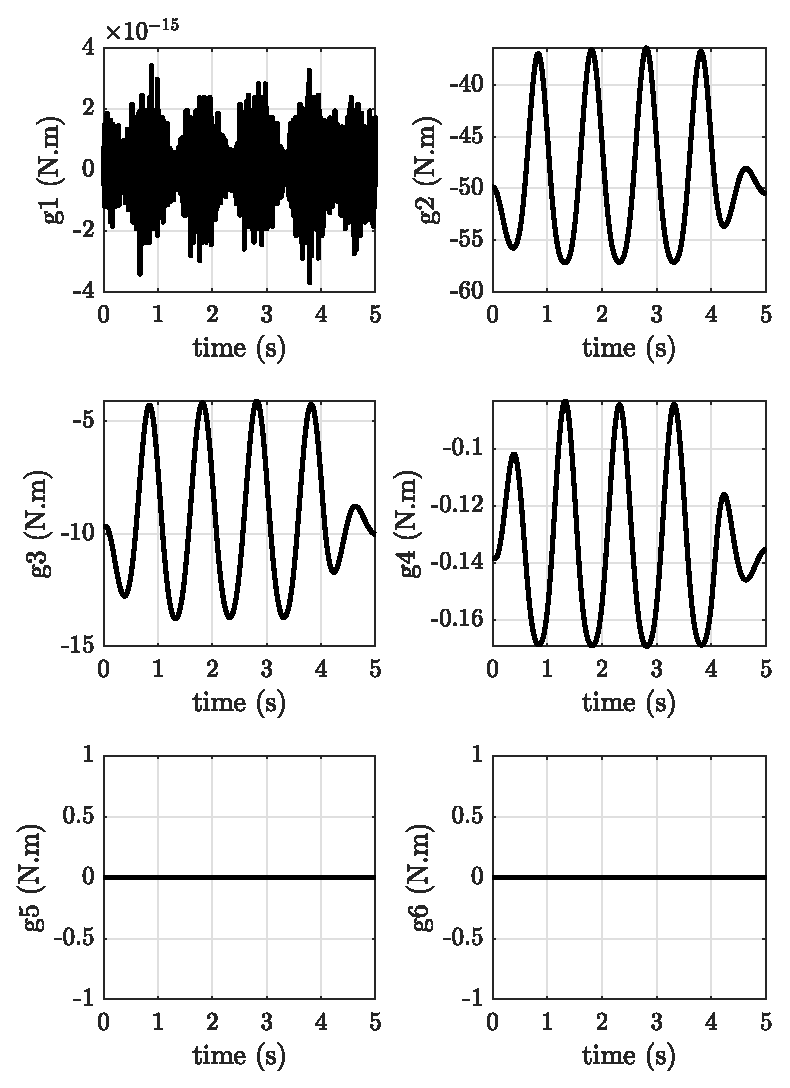
\includegraphics{images/act_1.6_sin/g.eps}
	\caption{The gravity term ($g$) of the PD with gravity compensation control method when the reference of second and fifth joints is a sinusoidal trajectory.}
	\label{fig:act_1.6_sin_g}
\end{figure}

